	\begin{enumerate}[label=\alph*)]
		\item	Tenemos que calcular la masa efectiva de los huecos para dos semiconductores diferentes, dado su densidad efectiva de estados en la banda de valencia. Esto significa que necesitamos invertir la fórmula típica, tal que
		      \begin{equation}
			      N_V = 2 \parentesis{\frac{m_p^* kT}{2\pi\hbar^2}}^{3/2} \quad \Rightarrow \quad m_p^* = \parentesis{\frac{N_V}{2}}^{2/3} {\frac{2 \pi \hbar^2}{kT}}
		      \end{equation}
		      De lo que se deduce que para el Si y el GsAs:

		      \begin{equation}
			      \text{Si:} \quad m_p^* = 7.38\cdot10^{-31} \text{kg} = 0.81 \ {m}_e
		      \end{equation}
		      \begin{equation}
			      \text{GaSi:}\quad m_p^* = 4.59 \cdot10^{-31} \text{kg} = 0.51 \ {m}_e
		      \end{equation}
		      Nivel intríseco 300K 1.7505319217070854
		\item Tenemos que calcular la posición del nivel intrínseco $E_i$ a la temperatura ambiente (300 K) y a 1000 $^\circ C$, asumiendo que $E_g$ es constante. Veamos que solo es aplicar una fórmula:
		      \begin{equation}
			      E_i = \frac{E_c+E_v}{2} + \frac{3}{4} kT \ln\parentesis{\frac{m_p^*}{m_n^*}}
		      \end{equation}
		      donde hemos considerado que $E_g=1.12$ en el silicio, y que $E_v=0$, ergo $E_c=1.12$. Hacemos la representación gráficamente. Las energías son: $300K: \ E_i=0.57$ eV y a 1273K $E_i: 0.70$ eV. Las masas usadas a 300K son: $m_p=0.81m_e$ y $m_n=1.18m_e$.
		      \begin{center}
			      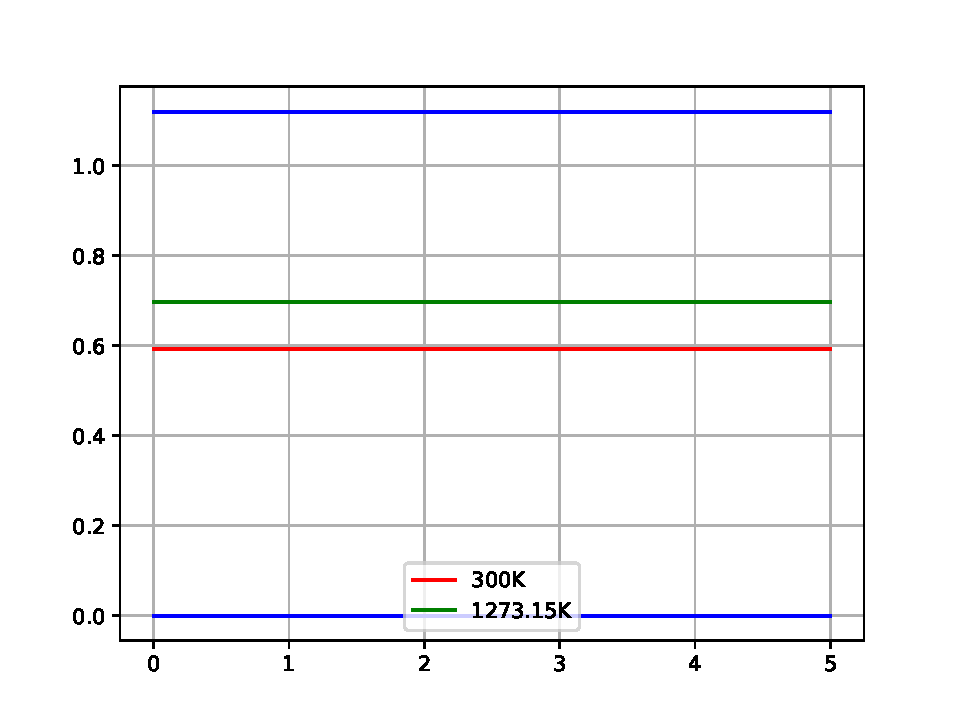
\includegraphics[width=0.6\textwidth]{Cuerpo/Ch_01/Ejercicio_01_5.pdf}
		      \end{center}
		      Viendo esta imagén no parece descabellado consdierar $E_i$ constante.
	\end{enumerate}
